\documentclass[11pt]{article}
\usepackage[margin=1in]{geometry}
\usepackage{amsmath,amssymb}
\usepackage{graphicx}
\usepackage{booktabs}
\usepackage{natbib}
\usepackage{xcolor}
\usepackage[hidelinks]{hyperref}
\usepackage{authblk}
\graphicspath{{figures/}}
\newcommand{\todo}[1]{\textcolor{red}{[\textbf{TODO:} #1]}}
\newcommand{\rms}{\mathrm{rms}}

\title{\bfseries The Training Dynamics of Massive Activations Are
Magnitude-Organized and Weight-Decay-Driven\\[2pt]
\large (working title --- sequel to \emph{Hidden Dynamics of Massive Activations})}
\author[1]{Aaron McClendon}
\author[1]{et al.}
\affil[1]{Arkitekt AI}
\date{Draft --- \today}

\begin{document}
\maketitle

\begin{abstract}
Massive activations (MAs)---a few hidden-state coordinates orders of magnitude
larger than the rest---emerge smoothly during training and are known to underwrite
attention sinks and stable gradient transport. Prior work established \emph{that}
they form (fitting a five-parameter law) and gave a one-sided lower bound: the MA
must be large enough to attenuate the sink gradient. We ask three dynamical
questions those results leave open---what ends the growth, whether the MA is
actively \emph{regulated}, and what it is \emph{for}---using small transformers
trained from scratch with dense checkpointing and causal weight-perturbation
experiments. We find: (i) the rise-and-decline is a \emph{global}
activation-scale phenomenon (nearly every sizeable channel follows the same
amplitude-parameterized shape), so the five-parameter law describes a global
dynamic and the MA is its large-amplitude tail; (ii) this turnover is
\emph{caused by weight decay}---with weight decay off the MA never turns over, and
the peak location is a near-log-linear function of the weight-decay coefficient
($\mathrm{corr}=-0.985$), a graded dose-response; weight decay drives the global
decline even at constant learning rate, with the decaying schedule amplifying it;
(iii) the gradient-attenuation floor operates on the
sink token's \emph{collective} $\rms$: the downstream gradient follows
$g\propto 1/\rms$ uniformly with the MA channel sitting exactly on that line
($0.94$ vs.\ $0.89$--$0.95$ for other large channels), confirming the mechanism of
\citet{chen2026gradient} while showing the MA is one contributor among several
(ablating it moves $\rms$ by only $\sim$5\%). Most notably, a battery of controls
shows that every apparent MA-specific property---a restoring ``floor'' and
``ceiling'' under displacement, a resistance to the global decline, and a
LayerNorm-gain dissociation---resolves into a \emph{magnitude} effect once compared
against equal-magnitude channels rather than random ones. \emph{Within these
measurements}, MAs are thus the extreme tail of magnitude-organized channel
dynamics rather than a distinct mechanism; we do not address the attention-bias
function documented elsewhere. A balance-condition theory (loss benefit vs.\ weight
decay) predicts the peak, and we show the decline localizes in per-weight
efficiency rather than weight shrinkage. Assembling these into a life cycle, we
further show that the MA's channel \emph{identity} is a stochastic role, not a fixed
dimension---different seeds place the sink on different channels (0/3 top-3 overlap
across seeds), decided by an early competition and locked in by step $\sim$4k; that
whether the MA \emph{stands apart} from a populated tail is a training-maturity
effect (a continuum early, becoming bimodal only late in training), which scopes the
equal-magnitude controls to the continuum regime; and that the late ``death'' of
losing channels is a competitive consolidation in which the sink concentrates onto a
redundant few. Of the mechanisms we test for that competition, three fail on
measurement (rms conservation, attention-sink saturation, and $1/\rms$ gradient
suppression); what survives is that AdamW's second-moment normalization---not raw
gradient magnitude, which is orders below the weight-decay pull---sustains the sink
cohort against decay, while \emph{which} channels win remains set by the early
stochastic lead.
\end{abstract}

\section{Introduction}

A trained transformer's hidden states are not uniform. In every model examined so
far, a handful of coordinates carry magnitudes hundreds or thousands of times the
typical activation, concentrated at a single token position and largely unchanging
across inputs \citep{sun2024massive}. These massive activations are not incidental:
they act as implicit attention biases, models degrade when they are removed, and
they are the principal obstacle to low-precision training and inference
\citep{dettmers2022llmint8,xiao2024streaming}.

Prior work gives a partial account. \citet{chen2026gradient} supply a mechanism for
why a large magnitude is useful --- it attenuates the gradient that accumulates at
an attention sink --- in the form of a lower bound the magnitude must clear.
\citet{gallego2025hidden} show that the emergence of massive activations over
training is highly regular, fitting a five-parameter law to their growth. These are
complementary but incomplete: one is a constraint and the other a curve. Neither
says what sets the magnitude in practice, what stops it growing, or why one
coordinate rather than another comes to carry it. We address those questions, and
the answer to the last turns out to govern how the first two should be read.

\paragraph{The identity of a massive activation is arbitrary.} If massive
activations were a structural feature of the architecture, the same coordinates
should carry them across independent runs. They do not. Retraining with a different
random seed --- same architecture, same data --- places the sink on entirely
different channels, with no overlap between the leading sets of any two seeds. The
number of such channels, the layer, and even the token position vary as well. What
does not vary is that \emph{some} small set wins: the phenomenon is structurally
inevitable, but the direction in which the symmetry breaks is not determined. The
winners are settled within the first few thousand steps and thereafter locked.

This reframes the object of study. A massive activation is not a privileged
dimension but a role, filled by whichever coordinates happen to lead an early
competition. It is also not a single unit: ablating the largest channel changes the
token's total magnitude by only a few percent, and the attention sink survives the
removal of any one of its carriers. The functional requirement identified by
\citet{chen2026gradient} is real, but it rests on the token's collective magnitude,
and any sufficient set of coordinates can supply it.

\paragraph{A life cycle.} The remaining results trace what happens to that role over
training. \emph{Birth}: a few channels win the early competition and lock in by step
${\sim}4$k, their identity seed-dependent (\S\ref{sec:stochastic}). \emph{Rise and
peak}: the winners grow alongside the surrounding field of large channels, until
loss-driven growth balances the pull of weight decay at a peak whose location and
height the decay coefficient sets (\S\ref{sec:decay},~\S\ref{sec:theory}).
\emph{Decline}: weight decay drives the magnitude down, though not by shrinking the
underlying weights, which continue to grow (\S\ref{sec:theory}).
\emph{Consolidation}: over a longer horizon the field erodes while the sink
concentrates onto a redundant few, so that a population which began as a smooth
continuum ends as a small set standing far above the rest
(\S\ref{sec:scale},~\S\ref{sec:birthdeath}).

\paragraph{Controlling for magnitude.} One methodological point runs through all of
this. Many properties look specific to the massive activation when it is compared
against an ordinary channel --- it is restored after ablation, it resists the
general decline, its normalisation gain behaves differently. But an ordinary channel
differs from the massive activation in size, so any such comparison confounds
identity with magnitude. The appropriate reference is a channel of comparable
magnitude, and the appropriate question is whether the massive activation departs
from the trend its own size predicts. Applied consistently
(\S\ref{sec:control-philosophy}), this control converts each of those apparent
effects into a magnitude effect. We report the hypotheses it eliminated alongside
those that survived.

\paragraph{Scope.} Two limits are worth flagging at the outset. Our claims concern
training dynamics and gradient attenuation; we do not study the attention-bias
function characterised by \citet{sun2024massive}, nor the finding that models
rebuild an outlier when architecturally denied one \citep{vemula}, both of which
operate at a level our experiments do not probe and both of which are consistent
with what we report. And the equal-magnitude control requires a populated band of
channels near the massive activation to serve as a reference. That band exists early
and mid-training and closes late (\S\ref{sec:scale}), so the deflations are claims
about the regime in which the control is well-posed, not about heavily-trained
frontier models.

\section{Background and related work}\label{sec:background}

\paragraph{Massive activations and attention sinks.} \citet{sun2024massive}
characterised massive activations as a small number of near-constant,
extreme-magnitude coordinates appearing at fixed feature dimensions and
predominantly at the first token or at delimiters. They function as implicit
attention biases: supplying the architecture with explicit learnable bias
parameters removes the need for them, and they do not form. The forward-side
counterpart is the attention sink \citep{xiao2024streaming} --- disproportionate
attention mass routed to an uninformative early token --- which
\citet{xiao2024streaming} exploit for streaming inference by retaining sink tokens
in the KV cache. \citet{darcet2023vision} report the same phenomenon in vision
transformers, where dedicated register tokens absorb it. A parallel, static line of
work documents outlier dimensions as an obstacle to quantisation
\citep{dettmers2022llmint8,kovaleva2021bert,bondarenko2023quantizable}.

\paragraph{The gradient-sink account.} \citet{chen2026gradient} give the mechanistic
account this paper builds on. Under causal masking, a token attended to by many
later positions also aggregates their gradients --- a gradient sink. Because the
normalisation Jacobian attenuates gradients in proportion to $1/\rms(x)$, a large
residual magnitude at that position suppresses the accumulated gradient. Their
Theorem gives a sufficient condition,
\begin{equation}\label{eq:bound}
\rms(x) \;\ge\; \frac{\lVert\gamma\rVert_\infty}{\tau}\,\lVert g_y\rVert
\;\Longrightarrow\;
\lVert\nabla_x\mathcal{L}\rVert \le \tau ,
\end{equation}
for any target gradient scale $\tau$. They test the implication with V-scale, a
modification attenuating gradient flow on the value path, and report that massive
activations are suppressed while attention sinks persist.

Two features of Equation~\eqref{eq:bound} shape what follows. It is stated on
$\rms(x)$, a property of the whole token rather than of any coordinate. And it is
one-sided: it establishes a floor and penalises nothing above it, so it predicts
neither a peak nor a decline.

\paragraph{Emergence over training.} \citet{gallego2025hidden} characterised the
developmental side, fitting the max-to-median ratio across 188 layers of the Pythia
suite with
\begin{equation}\label{eq:lognorm}
f(t) = A\,e^{-\lambda_{\mathrm{fit}} x_t}\log(x_t) + K,
\qquad x_t = \gamma t + t_0 ,
\end{equation}
at a mean $R^2$ of $0.984$, and predicting its parameters from architectural
features. The law has a critical point at which the ratio turns over, but the
mechanism producing it was left open.

\paragraph{What is new here.} Relative to \citet{chen2026gradient} we add the causal
and developmental layer --- weight decay as the driver of the trajectory --- and a
direct test of their bound's uniformity across channels, which confirms it and
establishes that the operative quantity is the token's collective $\rms$ rather than
any single coordinate. Relative to \citet{gallego2025hidden} we identify the
mechanism behind the critical point and reinterpret the law as describing
magnitude-organised channel dynamics generally. Relative to both, and to the outlier
literature, we show that which coordinates carry the phenomenon is a stochastic
outcome of training rather than a property of the network. We do not address the
attention-bias function or the architectural-robustness result of \citet{vemula};
those operate at a level our experiments do not probe.

\section{Preliminary}\label{sec:prelim}

This section fixes notation and defines the quantities the paper measures. Several
are closely related and can move in opposite directions, so we set them out
explicitly before using them.

\subsection{Architecture and hidden states}

We consider decoder-only transformers of $L$ pre-norm residual blocks. Block $\ell$
receives a hidden state $h_{\ell-1}\in\mathbb{R}^{S\times d}$ and returns
\begin{equation}
h_\ell = h_{\ell-1} + \mathcal{F}_\ell\!\left(\mathrm{Norm}(h_{\ell-1})\right),
\end{equation}
where $\mathcal{F}_\ell$ comprises multi-head self-attention and an MLP. We write
$h_\ell$ for the post-residual state --- the residual stream --- and index its
entries as $h_\ell(s,c)$ for token position $s$ and channel $c$. An
\emph{activation} is one such scalar. We do not examine intermediate quantities
inside $\mathcal{F}_\ell$ except where stated.

Two consequences of the pre-norm placement matter throughout. Sublayers see
normalised inputs, so the forward computation depends on the \emph{direction} of
$h_\ell$ at a position far more than on its scale: a coordinate can grow very large
without much altering what the next block computes. The backward pass is different.
The Jacobian of the normalisation carries a factor of order $1/\rms$, and that
factor is not normalised away. Residual magnitude is therefore close to free in the
forward direction and consequential in the backward one --- the asymmetry that makes
large activations useful rather than merely tolerable.

\subsection{The sink token}

Attention weights at each head are a softmax over positions and therefore sum to
one. When no position is worth attending to, the mass must still be assigned
somewhere, and it accumulates at a token carrying little content --- typically the
first, which under causal masking is the only position visible to every later one,
though delimiters also serve. We write $s^\ast$ for the sink position and measure
all quantities there unless otherwise noted. We identify $s^\ast$ per model as the
position carrying the largest activations rather than assuming position $0$, since
as we show it is not always position $0$ (\S\ref{sec:stochastic}).

\subsection{Three magnitudes}

Let $x = h_\ell(s^\ast,\cdot)\in\mathbb{R}^d$ be the sink token's hidden state at
layer $\ell$ and training step $t$. We use three quantities.

\paragraph{Channel magnitude.} $m_{\ell,t}(c) = |x_c|$, the value of a single
coordinate. This is what the perturbation experiments manipulate and what the
competition among channels is fought over.

\paragraph{Ratio.} Following \citet{gallego2025hidden},
\begin{equation}\label{eq:ratio}
r_{\ell,t} = \frac{\max_c|x_c|}{\mathrm{median}_c|x_c|},
\end{equation}
the max-to-median ratio, to which Equation~\eqref{eq:lognorm} was fitted. We retain
it for comparability with that work.

\paragraph{Root-mean-square.} $\rms_{\ell,t} = \sqrt{\tfrac{1}{d}\lVert x\rVert^2}$,
the token's aggregate scale, and the quantity appearing in
Equation~\eqref{eq:bound}. It is a property of the \emph{token}, not of any channel.

These three do not move together, and conflating them is the easiest way to misread
the phenomenon. In particular $r$ has a denominator that is itself changing: over
training the median falls, so $r$ can rise while the numerator $m$ of the dominant
channel is falling. We observe exactly this (\S\ref{sec:global}). Each claim below
is stated for a named quantity; where the emergence law is reinterpreted, it is
worth remembering that the law describes $r$ while the mechanisms we identify act on
$m$ and $\rms$.

\subsection{What counts as a massive activation}

\citet{sun2024massive} define an activation as massive when $|a| > 100$ and
$|a|/\mathrm{median}(|h_\ell|)\ge 1000$. As noted in \citet{gallego2025hidden},
these absolute thresholds do not transfer to smaller models, which exhibit the same
qualitative pattern at lower values, and we follow that work in identifying the
massive activation as the largest-magnitude channel at the sink of the layer where
$r$ is greatest.

This choice deserves emphasis rather than a footnote, because the paper's central
question is whether that channel constitutes a distinct category. Under a threshold
definition the question is settled by fiat; under ours, ``the massive activation''
names the argmax, and whether the argmax is a different kind of object or simply the
top of a continuous distribution becomes something to measure. We therefore also
report the \emph{isolation} of the leading channels: the largest ratio between
consecutive entries of the sorted magnitude profile at the sink. An isolation near
$1$ indicates a populated continuum in which the leader has close peers; a large
isolation indicates a small set standing apart from a collapsed bulk. We use
\emph{cohort} for the leading channels above that gap, without prejudging how many
there are.

\subsection{Gradient quantities}

The mechanism under test concerns the backward pass, so we measure gradients as well
as activations. We write $g$ for the gradient norm reaching the sink token at the
input to a block's normalisation --- the quantity Equation~\eqref{eq:bound}
constrains.

A channel is written into the residual stream by particular rows of the
output-projection matrices of the blocks below it. We call these the channel's
\emph{writer rows} and collect them as $w$. A channel's magnitude grows or shrinks
according to whether the loss-driven force on $w$ exceeds the pull of weight decay,
which we quantify by the \emph{maintaining force}
\begin{equation}\label{eq:maintain}
\mathrm{gp} \;=\; \frac{-\langle w,\hat g_w\rangle}{\lVert w\rVert^2},
\end{equation}
with $\hat g_w$ the gradient on the writer rows. Under AdamW the channel grows when
$\mathrm{gp} > \lambda$, the weight-decay coefficient, and erodes otherwise.

Two versions of Equation~\eqref{eq:maintain} appear below and they differ
substantially. The \emph{raw} maintaining force uses $\hat g_w$ directly. The
\emph{preconditioned} force applies AdamW's second-moment normalisation, dividing
each element by the square root of its accumulated squared gradient. Because a small
but persistent gradient has a correspondingly small second moment, preconditioning
can amplify it by orders of magnitude. As we show (\S\ref{sec:birthdeath}), the raw
force on every large channel falls far below $\lambda$ --- so the sink cannot be
sustained by raw gradient magnitude at all --- while the preconditioned force does
not. Statements about what maintains a channel must therefore be made after
preconditioning; instantaneous raw gradients do not read these dynamics.

\section{Method}\label{sec:method}

\subsection{Models and training}

We train decoder-only transformers from scratch at three scales, which we label by
their (weight-tied) parameter counts: 51M (8 layers, width 512, 8 heads), 203M
(12 layers, width 1024, 16 heads), and 380M (16 layers, width 1280, 16 heads). All
use context length 512, the GPT-2 byte-pair vocabulary (50{,}304 tokens), no bias
terms, learned positional embeddings, and tied input/output embeddings, and are
trained on the Dolma corpus. The primary model uses LayerNorm, with an RMSNorm
variant at matched configuration for architecture-generality. Optimisation uses
AdamW ($\beta=(0.9,0.95)$, gradient clipping at $1.0$) with weight decay
$\lambda=0.1$ and a peak learning rate of $6\times10^{-4}$ decayed by a cosine
schedule to $6\times10^{-5}$ after a linear warmup of 300 steps (400 for the two
larger models). The effective batch is 96 sequences of length 512 for the 51M model
(64 and 40 for the 203M and 380M models), in bfloat16. The three models train for
40k, 20k, and 10k steps, corresponding to approximately 2.0B, 0.7B, and 0.2B tokens.
Runs use seeds 1337 (primary) and 2024 (second seed). Checkpoints including optimiser
state are saved every 500 steps and activation probes recorded every 50 steps.
Training was performed on a single consumer GPU per run (NVIDIA RTX 4060 Ti, 16\,GB,
or RTX 4070 SUPER, 12\,GB).

For the identity, scale, and consolidation analyses we additionally use released
Pythia checkpoints \citep{biderman2023pythia} at 70M, 160M, 410M, 1.4B, 2.8B, and
6.9B parameters, including the seed re-runs at 70M, 160M, and 410M, and the
$\sim$150 intermediate training checkpoints released per model. These are analysed
by inference only; no Pythia model is trained or fine-tuned here.

\subsection{Probes}

Activations are measured at the sink position of each layer over a fixed batch of 24
sequences of length 512 from the validation split, held constant across checkpoints
so that trajectories are comparable (for Pythia, a fixed passage of held-out text).
At each probe we record the per-layer ratio $r$, the $\rms$ of the sink token, the
full ranked profile of channel magnitudes --- not only the argmax, so that
near-degeneracy between the leading channels is visible --- the identity of the
argmax channel and its layer, and the norms of the writer rows for the leading
channels.

\subsection{Perturbation protocol}

To ask whether a channel is actively maintained rather than passively accumulated,
we displace it and observe what training does. From a checkpoint we create forks
sharing batch order and a learning rate frozen at its value at the fork. In each
fork the target channel's writer rows are scaled by a factor $\alpha$ at every layer
--- single-layer intervention is insufficient, since the channel is written
redundantly across depth (\S\ref{sec:birthdeath}). We use $\alpha = 1$ as an
unperturbed control, which establishes how far two runs drift from data ordering
alone; $\alpha = 0$ to test for a restoring force from below; and $\alpha = 2$ to
test for one from above. Forks resume for 200--300 steps, with replicate resume
seeds where error bars are reported.

We report the perturbed fork's absolute trajectory alongside its gap to the control.
This matters because the control is itself moving during both the rising and
declining phases, so a closing gap does not by itself demonstrate that anything is
being restored. Recovery is summarised by the fraction of the initial gap closed
within the window and by the half-recovery time, which is more robust than an
exponential time constant when the return is not single-exponential.

\subsection{Controlling for magnitude}\label{sec:control-philosophy}

The perturbation protocol answers whether a channel responds; it does not answer
whether the response is peculiar to \emph{that} channel. A randomly chosen channel
differs from the massive activation in magnitude, so comparing the two confounds
identity with size. Since almost every quantity we measure varies with magnitude,
that confound is not incidental --- it is the default outcome.

We therefore compare against equal magnitude wherever the comparison is available,
by three means. First, we regress the property of interest on channel magnitude and
ask whether the massive activation departs from that trend, scoring it out-of-sample
against a trend fitted to the bulk rather than by leave-one-out; adjacent
high-magnitude channels otherwise distort each other's fits, which we show can
manufacture an apparent outlier where none exists (\S\ref{sec:controls}). Second, we
match perturbations for the change they induce in $\rms$, so that a single-channel
displacement and one distributed across many channels are comparable. Third, we pool
across layers, architectures, and seeds, and require at least 10 channels per group
before reporting any differentiator, having twice found clean separations at smaller
samples dissolve under proper sampling.

This control has a precondition, examined in \S\ref{sec:scale}: there must exist
channels of comparable magnitude to serve as the reference. Whether they do is a
property of the training regime rather than a fixed fact about transformers.

\section{Massive activations emerge and follow a global law}\label{sec:global}
The max/median \emph{ratio} of the dominant layer follows the five-parameter law
with $R^2=0.999$ over 40k steps (Fig.~\ref{fig:emergence}), reproducing
\citep{gallego2025hidden}. The ratio and the raw \emph{magnitude} can disagree in
direction: at layer 5 the ratio rises monotonically (to $\sim$400) while the
underlying MA magnitude peaks near step 20k and declines, because the median falls
faster than the MA. This distinction matters throughout---the law was fit to the
\emph{ratio}, whereas the weight-decay mechanism below acts on the \emph{magnitude},
the two linked by the falling median---so we name the quantity for each claim.
Measuring per-channel \emph{magnitudes} directly (Fig.~\ref{fig:global}a, layer 2),
essentially every sizeable channel rises then declines (98/98 at layer 2; 382/398
at layer 5), and the peak \emph{location} tends to increase with amplitude
(Fig.~\ref{fig:global}b), small channels peaking early and large ones late, the MA
at the extreme---though the relation is noisy and right-censored (caption). The
magnitude dynamics are thus \emph{global} and amplitude-organized; nothing about
the shape is MA-specific, and the five-parameter ratio law reflects both this
magnitude dynamic and the falling median.

\begin{figure}[t]\centering
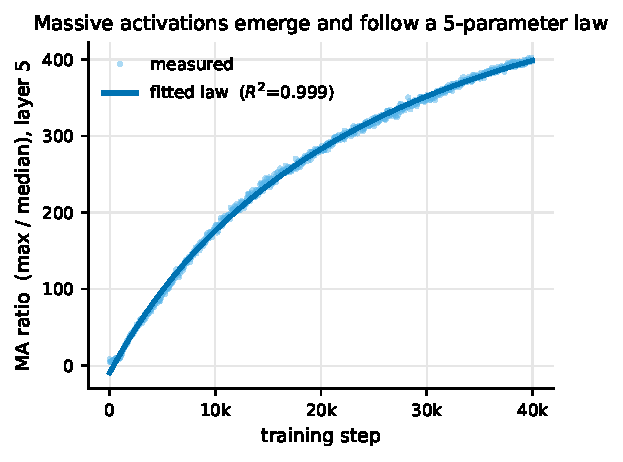
\includegraphics[width=0.6\linewidth]{fig1_emergence.pdf}
\caption{MAs emerge and fit the five-parameter law of \citep{gallego2025hidden}
($R^2=0.999$; layer 5, 51M model).}\label{fig:emergence}
\end{figure}
\begin{figure}[t]\centering
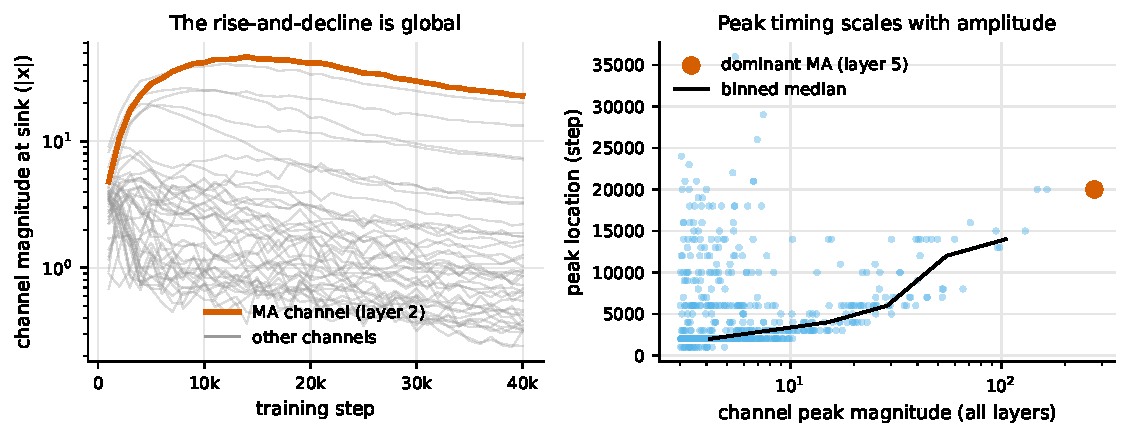
\includegraphics[width=\linewidth]{fig2_global_dynamic.pdf}
\caption{\textbf{The rise-and-decline is global.} (a) Per-channel sink magnitude
(layer 2): nearly all sizeable channels rise then decline; the MA is the
large-amplitude tail. (b) Peak location vs.\ channel peak magnitude, pooled over
layers; the binned median (line) rises with amplitude, but the per-channel scatter
is wide at any amplitude and \emph{right-censored}---channels peaking beyond the
40k-step window cannot appear, biasing the high-amplitude end downward---so we read
a tendency, not a clean law.}\label{fig:global}
\end{figure}

\section{Weight decay causes the turnover}\label{sec:decay}
Continuing from a near-peak checkpoint with weight decay \emph{off}, the global
activation scale (median $|x|$) keeps rising---no turnover; with weight decay on it
declines, and it declines \emph{even at constant learning rate} ($-11\%$ over the
compared window vs.\ $-18\%$ under the decaying schedule; Fig.~\ref{fig:decay}a).
Weight decay is thus necessary for the turnover and drives the decline; the
decaying schedule \emph{amplifies} the decline rather than causing it. (We read the
causal effect on the global median: the single MA channel is noisier, plateauing
rather than declining at constant LR, so the constant-LR effect is clearest at the
population scale.) Sweeping $\lambda$ under the schedule moves the MA peak location
near log-linearly, $t_{\text{peak}}\approx a-b\ln\lambda$ ($\mathrm{corr}=-0.985$;
Fig.~\ref{fig:decay}b); at $\lambda=0$ there is no peak, and the peak magnitude
scales as $\lambda^{-1/2}$ (\S\ref{sec:theory}). The turnover of the MA magnitude
is thus set by, and movable with, the weight-decay coefficient.

\begin{figure}[t]\centering
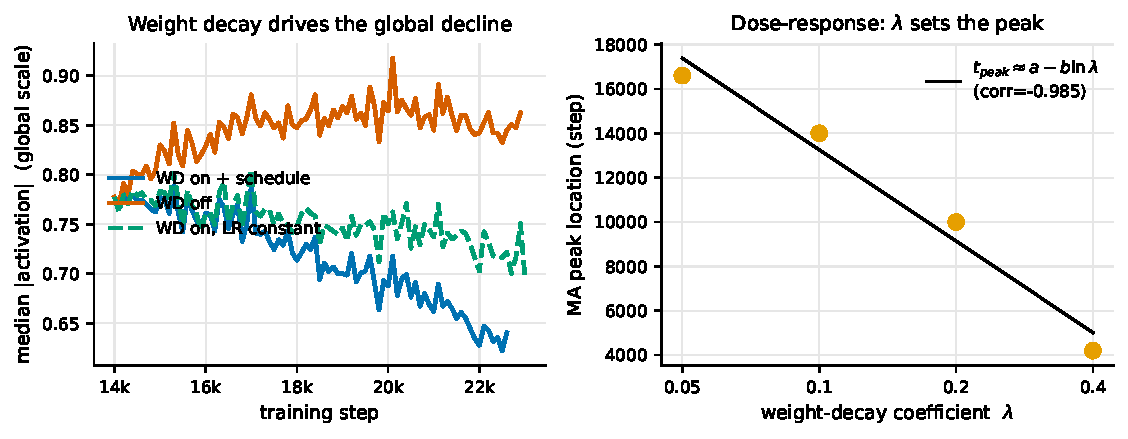
\includegraphics[width=\linewidth]{fig3_weight_decay.pdf}
\caption{\textbf{Weight decay causes the turnover.} (a) Global scale (median
$|x|$): weight decay off $\to$ rises (no turnover); on $\to$ declines; constant-LR
declines less than the schedule, so the schedule \emph{amplifies} rather than
causes the decline. (b) Near-log-linear dose-response of the MA peak location vs.\
$\lambda$, under the schedule ($\mathrm{corr}=-0.985$).}\label{fig:decay}
\end{figure}

\section{The gradient floor is on the token's collective $\rms$}\label{sec:floor}
The gradient-sink bound predicts the downstream sink gradient $g$ should scale as
$1/\rms(x)$. Ablating channels (reducing $\rms$) should raise $g$ in proportion. We
ablate the MA and several other large channels individually and measure $(\rms,g)$
at the sink (one forward+backward each, no training). The product $g\cdot\rms$ is
constant across all conditions, and the MA is \emph{not} an outlier: its
$g/(1/\rms)$ ratio is $0.94$, squarely within the $0.89$--$0.95$ of the other large
channels (Fig.~\ref{fig:controls}a). This is a clean, positive confirmation of
\citep{chen2026gradient}. It also sharpens it: ablating the MA moves $\rms$ by only
$\sim$5\%, so the MA is one of several comparable contributors, and the quantity the
mechanism reads is the token's \emph{collective} $\rms$---``the MA does gradient
attenuation'' is imprecise; the token's $\rms$ does, and the MA is part of it.

\section{Apparent MA-specific regulation resolves to magnitude}\label{sec:controls}
Perturb-and-restore experiments initially suggested MA-specific regulation: an
ablated MA is rebuilt (a floor) while an over-driven MA is pulled back in the
declining regime (a ceiling), each far more than a matched-\emph{norm} random
channel, and decay-independent. But a random channel differs from the MA in
magnitude; the proper control is equal magnitude.

\paragraph{The ceiling is $\rms$-, not direction-, driven, and is a large-channel
effect.} Matched-$\rms$ displacements that distort the sink direction $\hat x$
(scaling the MA alone) versus preserve it (scaling the top channels
proportionally) are pulled back \emph{equally} (73\% vs.\ 71\% of the $\rms$ excess
removed) despite an $11\times$ difference in $\hat x$ distortion
(Fig.~\ref{fig:controls}b). And a proportional kick to the top-16 channels is
pulled back nearly as much as the MA (71\% vs.\ 73\%), whereas a small random
channel is not ($\sim$20\%). The ceiling tracks perturbation magnitude, not the MA.

\paragraph{The gain dissociation is not an MA-specific outlier.} On the unperturbed
trajectory the MA preserves its magnitude while its LayerNorm gain $\gamma$
collapses. Regressing this dissociation against magnitude, the gain is \emph{not}
magnitude-organized (per-layer slopes range $-10$ to $+52$, sign-changing), yet the
apparent MA outlier does not survive a clean baseline: fitting the trend on the bulk
of channels and scoring the top ranks out-of-sample, the MA sits at
$z=+0.31$ (4/8 conditions positive)---on its magnitude trend, not above it. The
residual $z=+1.46$ from a naive leave-one-out was manufactured by the
high-magnitude runner-up channels depressing each other's fitted trends. What
remains is a weaker, noisier structural note: the LayerNorm gain of large channels
is not organized by magnitude and shows scattered, partly initialization-dependent
reallocation.

\begin{figure}[t]\centering
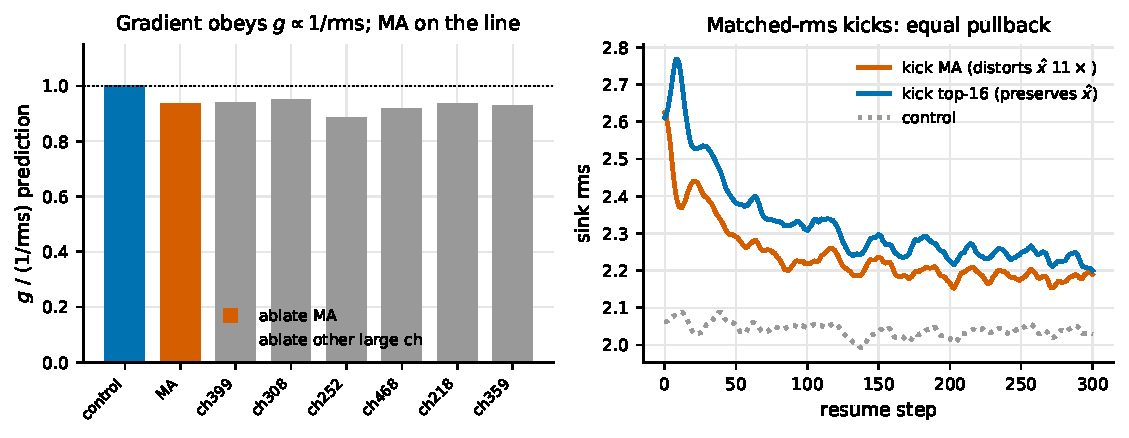
\includegraphics[width=\linewidth]{fig4_controls.pdf}
\caption{\textbf{Controls: apparent MA-specificity resolves to magnitude.}
(a) The downstream sink gradient obeys $g\propto1/\rms$ uniformly ($g\cdot\rms$
constant); the MA lies on the line with the other large channels---confirming the
gradient bound, and locating it on collective $\rms$. (b) Matched-$\rms$
displacements are pulled back equally regardless of direction distortion; the
declining-regime ``ceiling'' is a large-channel, $\rms$ effect.}\label{fig:controls}
\end{figure}

\section{The massive activation is a stochastic role, not a fixed dimension}\label{sec:stochastic}
If the MA were a distinguished structural feature of the network, the same coordinate
should carry it across independent training runs. It does not. Re-training with a
different random seed---same architecture, same data---moves the MA to a different
channel. In our 51M model the dominant sink is channel 207 under one seed and 263
under another; across three seeds of Pythia-410m the top-three sink channels share
\emph{no} members (Table~\ref{tab:seed}). The number of sink channels (one to three),
the birth layer, and even the sink token position all vary by seed. ``Which channel
is the MA'' is therefore set by early stochastic symmetry-breaking, not by the
architecture or the data.

\begin{table}[t]\centering\small
\begin{tabular}{lll}
\toprule
model & seed & top-3 sink channels\\
\midrule
ours (51M) & 1337 & 207, 399, 308\\
ours (51M) & 2024 & 263, 114, 399\\
Pythia-410m & default & 357, 130, 966\\
Pythia-410m & seed 1 & 110, 345, 27\\
Pythia-410m & seed 2 & 424, 584, 216\\
\bottomrule
\end{tabular}
\caption{\textbf{Sink identity is seed-stochastic.} Same architecture and data,
different RNG seed. The three Pythia-410m seeds share no top-3 channels (0/3 overlap
for every pair); our two 51M seeds share only a secondary channel.}\label{tab:seed}
\end{table}

The winner is decided \emph{early} and then locked (Fig.~\ref{fig:lockin}). Tracking
channel magnitude rank across training in Pythia-410m, the eventual top three occupy
ranks 1--3 from step $\sim$4k---a small fraction of the 143k-step run---and never
relinquish them; the rank at step 8k already predicts the rank at 143k (Spearman
$\approx+0.5$ to $+0.7$), with a sharp cutoff just below the surviving set (a channel
sits perpetually at rank~4, never joins the winners, and later collapses in
magnitude). The same lock-in holds in our own 51M model, where we can watch the
birth directly: the argmax coordinate migrates over the first few thousand steps
(ch221$\to$ch308$\to$ch207) and then locks to ch207 by step $\sim$5k for the
remainder of training (Fig.~\ref{fig:lockin}b)---an explicit early
symmetry-breaking. The identity is also input-robust: the same channels carry the
sink across ten unrelated text passages (10/10 identical top-3). This reframes
MA-specificity at the level of \emph{identity}: the MA is a role a channel wins in an
early competition, not a privileged coordinate. It sharpens the outlier-feature
literature
\citep{dettmers2022llmint8,kovaleva2021bert}---outlier dimensions exist robustly, but
\emph{which} coordinates are outliers is a stochastic outcome of training.

\begin{figure}[t]\centering
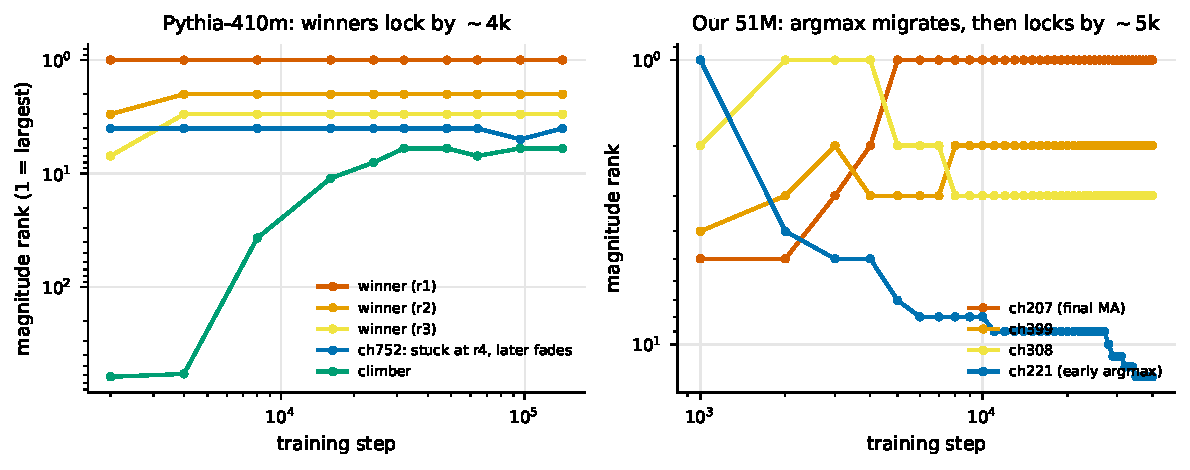
\includegraphics[width=\linewidth]{fig9_lockin.pdf}
\caption{\textbf{Early lock-in of the sink channels.} Magnitude rank vs.\ training
step (rank 1 = largest; log axes). (a) Pythia-410m: the three winners settle at ranks
1--3 by step $\sim$4k and never move; the rank-4 channel sits just below the cut
(its magnitude later collapses, Fig.~\ref{fig:dropout}); a climber rises from
obscurity. (b) Our 51M: the argmax coordinate migrates (ch221$\to$ch308$\to$ch207)
before locking to ch207 by step $\sim$5k---the birth of the MA as early stochastic
symmetry-breaking.}\label{fig:lockin}
\end{figure}

\section{Scale and training maturity set whether the MA stands apart}\label{sec:scale}
The equal-magnitude control (\S\ref{sec:controls}) presupposes a populated band of
channels comparable to the MA. Whether that band exists is itself a function of scale
and training maturity. We measure the sorted per-channel magnitude profile at the
sink, across our from-scratch family (51M--380M) and Pythia (70M--6.9B)
(Fig.~\ref{fig:scale}).

Two facts emerge. First, the MA's separation from the typical channel (max/median)
grows monotonically with scale in \emph{both} families (ours $195\to382$ over
51M$\to$380M; Pythia $138\to1693$ over 70M$\to$6.9B), and our from-scratch models sit
squarely on the Pythia trend---they are not anomalous in how extreme the MA becomes.
Second, the \emph{shape} of the tail differs by regime: our lightly-trained models
are a smooth, populated continuum (largest consecutive-rank drop $<2.5\times$, even
at 380M), whereas trained Pythia models are bimodal---a few giant channels on a cliff
above a collapsed bulk.

This is a \emph{training-maturity} effect, not a parameter-count one. Following a
single Pythia-410m through training, the profile is a continuum early---at step 16k
the cliff is $1.7\times$, indistinguishable from our models---and the bimodal cliff
grows with tokens to $16.8\times$ by 143k (Fig.~\ref{fig:scale}b). At matched
maturity even a 410M model resembles our 51M. The equal-magnitude control is thus
well-posed in the continuum regime (early/mid training, where our from-scratch models
and early Pythia live); at frontier maturity the MA has few magnitude-matched peers
and the control is harder to pose. \emph{We scope the deflations of
\S\ref{sec:controls} to the continuum regime.} Finally, the MA's magnitude separation
\emph{saturates} by $\sim$32k while the bimodal isolation keeps rising to 143k
(Fig.~\ref{fig:scale}c): magnitude growth and structural isolation are decoupled, and
the late isolation is a distinct process we turn to next.

\begin{figure}[t]\centering
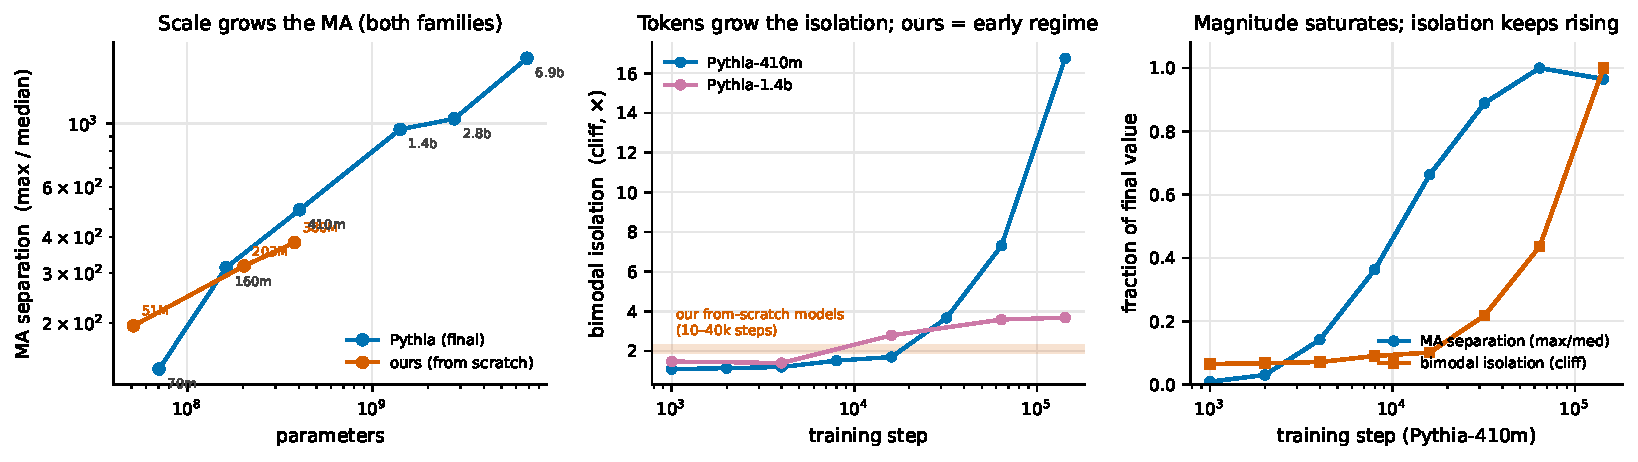
\includegraphics[width=\linewidth]{fig5_scale.pdf}
\caption{\textbf{Scale grows the MA; training tokens isolate it.} (a) max/median
separation grows with scale in both families; our from-scratch models lie on the
Pythia trend. (b) In a single Pythia-410m, the bimodal isolation (largest
consecutive-rank drop) is $\sim$1 early---a continuum, like our models---and grows
with training tokens to $\sim$17$\times$; the shaded band marks our from-scratch
models. (c) Magnitude separation saturates early while isolation keeps
rising---decoupled processes.}\label{fig:scale}
\end{figure}

\section{Birth and death: competitive consolidation of the sink}\label{sec:birthdeath}
The continuum-to-bimodal transition is the visible trace of a competition among large
channels: a few win and are maintained while the rest---including channels briefly
comparable to the winners---collapse. We characterize this ``birth and death'' and,
importantly, separate the parts we can explain from the parts we cannot.

\paragraph{The winners grow, the field is stripped, and the two are not conserved.}
Following the sink vector of Pythia-410m from step 16k to 143k
(Fig.~\ref{fig:dropout}), the surviving channels rise then decline mildly---the
balance-law trajectory of \S\ref{sec:theory}---while the mid-rank channels erode
monotonically and \emph{staggered}, each on its own schedule with no synchronized
transition. The energy fraction carried by the top three rises from $0.55$ to $0.99$.
This is not a conservation law: total sink $\rms$ peaks and declines rather than
holding flat, and the winners' energy gain exceeds the field's loss by $\sim$3$\times$.
The winners grow on their own loss-driven trajectory; they do not merely inherit the
field's magnitude. In our 51M model, which stays in the continuum regime
(\S\ref{sec:scale}), the same decline is \emph{graded} rather than selective: ranking
channels by peak magnitude, retention from peak to end falls smoothly with rank
($0.89, 0.88, 0.85, 0.83, 0.80, 0.83, 0.82, 0.78$ for the top eight), the MA
\emph{on} this ladder rather than above it. The magnitude-organized reading of
\S\ref{sec:controls} thus holds wherever a populated tail exists; the sharply
selective, winner-take-most consolidation is the same competition run to maturity.

\paragraph{The sink is a redundant collective.} Ablating any single surviving channel
barely changes the attention paid to the sink token ($0.004$--$0.015$), but ablating
the top three together removes far more ($0.08$, $\sim$3$\times$ superadditive), while
random channels do nothing (Fig.~\ref{fig:redundancy}). The sink is jointly and
redundantly implemented, consistent with the collective-$\rms$ reading of the floor
(\S\ref{sec:floor}) and with attention-sink accounts
\citep{sun2024massive,xiao2024streaming}; it also explains why single-channel
ablations are weak (\S\ref{sec:method}).

\begin{figure}[t]\centering
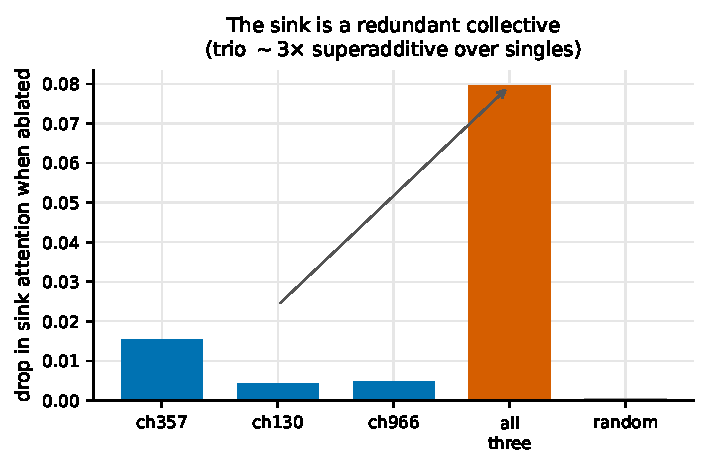
\includegraphics[width=0.46\linewidth]{fig10_redundancy.pdf}
\caption{\textbf{The sink is a redundant collective.} Drop in attention to the sink
token when residual channels are ablated (Pythia-410m, step 16k). Each surviving
channel alone matters little; the three together are $\sim$3$\times$ superadditive;
a random channel does nothing.}\label{fig:redundancy}
\end{figure}

\paragraph{What drives the competition---mostly refuted on measurement.} We tested
the natural mechanisms and most fail, which we state plainly. (i)~The gradient floor
does \emph{not} erode the field by $1/\rms$ suppression: the writer-row gradient on a
collapsing channel does not fall as $1/\rms$ (the product $g\cdot\rms$ \emph{rises}),
and collapsing channels receive as much gradient as surviving ones. (ii)~The survivor
\emph{count} is not set by attention-sink saturation: across seed re-runs at fixed
scale (70M, 160M) it does not track total sink attention (corr $\approx0$); the count
is itself stochastic. (iii)~There is no rms-conservation constraint (above). What
\emph{is} measurable is one cohort-level fact about how the sink survives weight decay
at all: the raw maintaining gradient on \emph{every} large channel is one-to-two
orders of magnitude below the weight-decay pull ($\sim\!10^{-4}$ vs.\
$\lambda=10^{-2}$), so the sink cannot be sustained by raw gradient magnitude. It is
sustained by AdamW's second-moment normalization, which amplifies a persistent
sub-decay gradient: the Adam-preconditioned maintaining force is positive for the
large-channel cohort and near zero for random channels (Fig.~\ref{fig:adam}). The
maintenance thus lives in optimizer preconditioning---the positive form of our
earlier negative that the regulation is invisible to instantaneous raw gradients
(\S\ref{sec:theory}). Table~\ref{tab:refuted} summarizes the tested mechanisms.

\begin{figure}[t]\centering
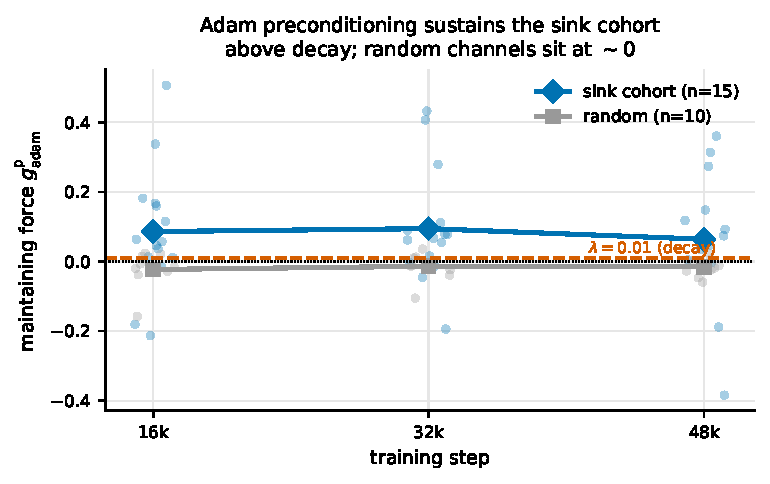
\includegraphics[width=0.6\linewidth]{fig7_adam.pdf}
\caption{\textbf{Adam preconditioning sustains the sink cohort against decay.}
Adam-preconditioned maintaining force $g^{\mathrm{p}}_{\mathrm{adam}}=-\langle w,
m/\sqrt v\rangle/\lVert w\rVert^2$ over three checkpoints; a channel's writer norm
grows iff this exceeds the weight decay $\lambda=0.01$ (dashed). The sink cohort
(winners$+$collapsers) sits above the decay line; random channels sit at $\sim$0. The
raw (un-preconditioned) force is $\sim\!10^{-4}$ for \emph{all} channels---two orders
below decay---so the maintenance is an optimizer-preconditioning effect. The cohort
is separated from random, but winners are \emph{not} separated from collapsers (wide
overlap), consistent with selection being unresolved.}\label{fig:adam}
\end{figure}

\begin{table}[t]\centering\small
\begin{tabular}{p{3.4cm}p{3.5cm}p{4.2cm}l}
\toprule
hypothesis & prediction & measurement & verdict\\
\midrule
MA-specific restoring force & restores more than an equal-magnitude channel &
matched-$\rms$ kicks pulled back equally (\S\ref{sec:controls}) & refuted\\
rms conservation & total sink $\rms$ flat; winner gain $=$ field loss &
$\rms$ peaks-and-declines; gain/loss $=2.9$ & refuted\\
softmax saturation sets count & survivor count tracks sink attention &
corr $\approx 0$ across seed re-runs & refuted\\
$1/\rms$ suppression erodes field & writer gradient falls as $1/\rms$ &
$g\cdot\rms$ \emph{rises} $1.5$--$2\times$; collapsers $\approx$ winners & refuted\\
\midrule
Adam preconditioning sustains cohort & preconditioned force $>\lambda$ for cohort,
$\sim\!0$ random & holds; raw force $\sim\!10^{-4}\ll\lambda$ (Fig.~\ref{fig:adam})
& supported (cohort)\\
\bottomrule
\end{tabular}
\caption{\textbf{Mechanisms tested for the competition.} Four candidate mechanisms
are refuted on measurement; one cohort-level fact survives. \emph{Which} channels win
(intra-cohort selection) remains unresolved.}\label{tab:refuted}
\end{table}

\paragraph{What is not explained.} \emph{Which} cohort members ultimately win is set
by the early stochastic lead (\S\ref{sec:stochastic}); we could not measure a
mechanistic selector distinguishing survivors from equal-cohort collapsers. The
preconditioned maintaining force separates the sink cohort from random channels but
does \emph{not} separate winners from collapsers (a genuine survivor can show a
negative maintaining force on held-out text), indicating the selection is not
readable from post-hoc gradients on a different corpus. Resolving it would require the
training-time optimizer state, absent from released checkpoints. We leave this as an
explicit open question rather than over-claim a mechanism the data does not support.

\begin{figure}[t]\centering
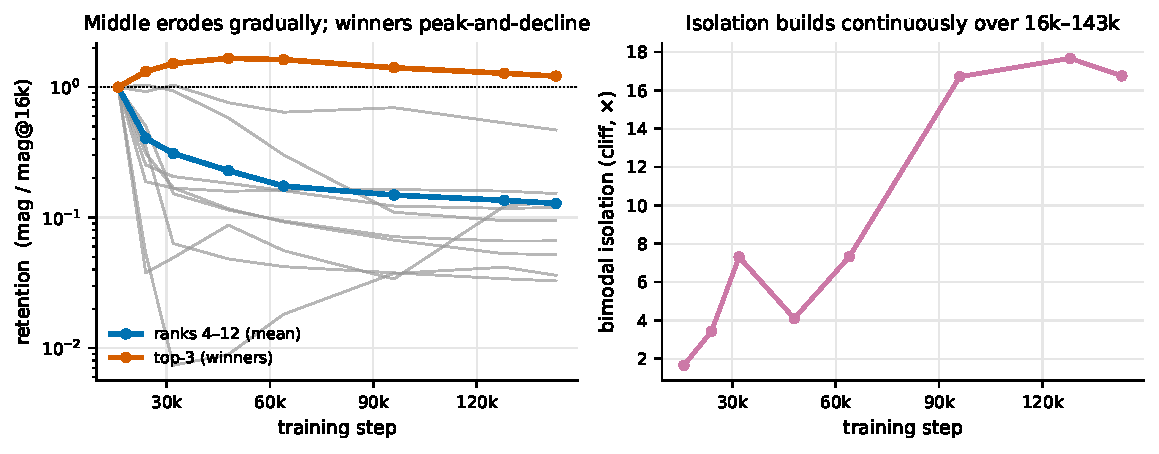
\includegraphics[width=\linewidth]{fig6_dropout.pdf}
\caption{\textbf{Competitive consolidation (Pythia-410m, 16k$\to$143k).} (a) The
top-3 winners rise then decline mildly while mid-rank channels erode gradually and
staggered---no synchronized transition. (b) The bimodal isolation builds continuously
over the window; there is no single onset step.}\label{fig:dropout}
\end{figure}

\section{Theory: a balance condition, and where the decline lives}\label{sec:theory}
Let $w$ be the aggregate writer weights feeding the MA channel; to leading order the
MA magnitude $m\propto\lVert w\rVert$. Under AdamW, $w_{t+1}=w_t-\eta(\hat g_t+
\lambda w_t)$, so $\tfrac{d}{dt}\lVert w\rVert^2\approx-2\eta(\langle w,\hat
g\rangle+\lambda\lVert w\rVert^2)$ and the MA peaks when
\begin{equation}
G(t^\ast)=\lambda\,\lVert w(t^\ast)\rVert,\qquad G\equiv-\langle\hat w,\hat g\rangle,
\end{equation}
the loss-driven growth force balancing the decay pull---an equality complementing
the inequality of \citep{chen2026gradient}. With a power-law marginal benefit
$G(m)=c\,m^q$, one gets $m_{\text{peak}}\propto\lambda^{-1/(1-q)}$; the measured
peak-magnitude scaling ($\propto\lambda^{-1/2}$; slope $-0.51$ to $-0.57$ across
estimators, Fig.~\ref{fig:balance}b) fixes $q=-1$, a
logarithmic benefit $B(m)\propto\log m$, which also explains why the loss force is
tiny (order $1/m$) at large $m$. Directly measured, $\lVert w\rVert$ grows as
$\sqrt t$ pre-peak (not exponentially), the balance $G=\lambda\lVert w^\ast\rVert$
holds, and $G$ falls over training (Fig.~\ref{fig:balance}a).

\begin{figure}[t]\centering
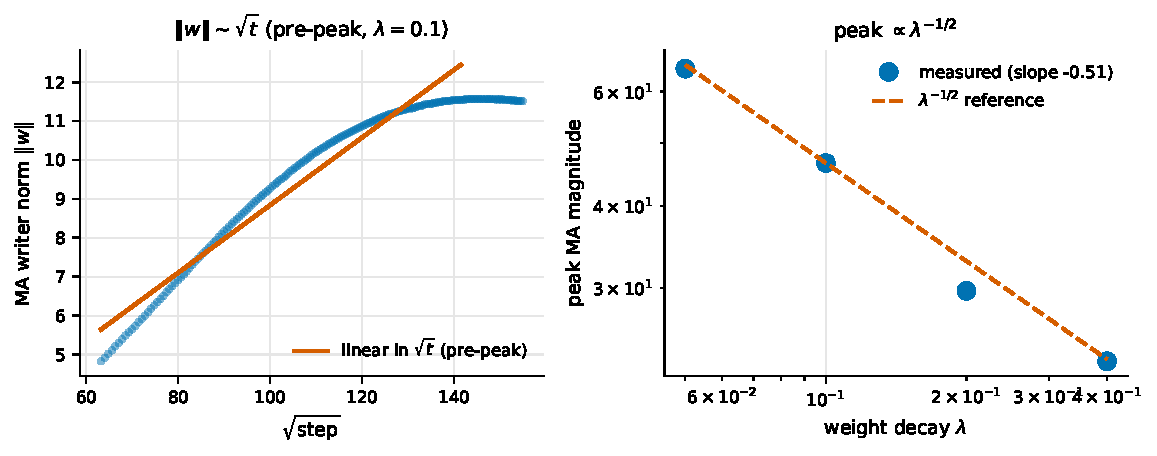
\includegraphics[width=\linewidth]{fig8_balance.pdf}
\caption{\textbf{The balance-condition theory.} (a) The MA writer norm $\|w\|$ grows
linearly in $\sqrt{t}$ pre-peak (not exponentially), then bends over as the balance
$G=\lambda\|w\|$ is reached ($\lambda=0.1$). (b) The peak MA magnitude scales as
$\lambda^{-1/2}$ across a weight-decay sweep (measured slope $-0.51$), fixing the
marginal-benefit exponent $q=-1$.}\label{fig:balance}
\end{figure}

\paragraph{The decline is a per-weight efficiency change, not weight shrinkage.} A
striking measurement: at baseline weight decay the MA magnitude turns over
\emph{while its writer weights keep growing} (e.g.\ at $\lambda=0.1$, $\lVert
w\rVert$ rises $10.8\to11.5$ across the activation's decline while $m/\lVert
w\rVert$ falls $4.2\to3.2$); only at strong decay does $\lVert w\rVert$ itself
shrink. So the decline lives in the per-weight efficiency---a representational
reorganization---rather than in the weight norm. We do not claim ``weight decay
shrinks the MA weights.''

\paragraph{Scope of the balance law.} The ODE above rests on $m\propto\lVert
w\rVert$ and describes the \emph{rise and peak}, where it is calibrated (via the
$\lambda$-sweep of the peak). It does \emph{not} govern the decline: that
proportionality breaks there ($\lVert w\rVert$ grows while $m/\lVert w\rVert$ falls,
above), so the fractional-decline prediction of the single-channel $G(m)=c\,m^q$ does
not carry over to the declining, multi-channel population. In particular the
cross-channel retention ordering during the decline (larger channels retained more;
\S\ref{sec:birthdeath}) is a competition phenomenon of the decline regime, not a
consequence of the balance ODE, and $q=-1$ is fixed by the MA's \emph{own}
peak-scaling rather than being a universal cross-channel law. The balance condition
and the competitive consolidation are two accounts at two stages of the life cycle,
and we do not conflate them.

\paragraph{Honest negatives, and their positive form.} We could not read the
regulation off instantaneous \emph{raw} gradients (activation- or weight-space,
multi-batch averaged); the signal is below chance and entangled with Adam
preconditioning. \S\ref{sec:birthdeath} turns this into a quantitative statement: the
raw maintaining gradient is one-to-two orders below the weight-decay pull at every
large channel, so the sink is held up not by raw gradient magnitude but by AdamW's
second-moment normalization---the regulation is an emergent optimizer-preconditioning
effect, visible under displacement or after preconditioning but not in the raw
gradient. A direction test did not isolate a representational cost for the ceiling.

\section{Discussion}
\paragraph{The life cycle, assembled.} A massive activation is born when a few
channels win an early, seed-dependent competition to carry the sink and lock in by
step $\sim$4k; it rises with the surrounding field of large channels along an
amplitude-organized law; it peaks where loss-driven growth balances the weight-decay
pull, at a location and height the decay coefficient controls; it declines as a
per-weight-efficiency reorganization once weight decay dominates; and over a long
horizon it is the survivor of a competitive consolidation that strips the field and
concentrates the sink onto a redundant few. Throughout, the object doing the work is
the token's collective $\rms$, not a singular channel, and the carrier's identity is
arbitrary. The one force we can measure sustaining the sink against decay is not raw
gradient magnitude---which is orders below the decay pull---but AdamW's second-moment
normalization; \emph{which} channels win the competition is set earlier and
stochastically, and its mechanism we leave open. Four tempting mechanistic
hypotheses (an MA-specific restoring force, rms conservation, attention-sink
saturation, and $1/\rms$ suppression of the field) each died on measurement, and the
account is stronger for their falsification than it would be with any of them assumed.

\paragraph{What is magnitude-organized, and what we claim.} The training dynamics
(emergence shape, the weight-decay-driven rise-and-fall) and the gradient
attenuation ($g\propto1/\rms$) of outlier channels are magnitude-organized; within
our measurements every apparent MA-specific regulation deflated to a magnitude
effect once controlled against equal-magnitude channels. Two relationships are
worth contrasting: attenuation is tightly magnitude-organized with the MA
\emph{on the line}, while the LayerNorm gain has no magnitude law at all. Whatever
would single out the MA is not its size---but our controls did not find that
something in the dynamics or attenuation.

\paragraph{Scope and what we do not address.} This is a claim about our
measurements, not a universal. We do not study the attention-bias function
\citep{sun2024massive} or the rebuild-when-denied-a-home result \citep{vemula},
both of which remain consistent with the MA behaving as a functional unit at a
level our experiments do not probe. The equal-magnitude deflations are scoped to the
\emph{continuum regime} (early/mid training, where a populated tail exists); we do
not claim they transfer to the bimodal, late-training regime of heavily-trained
frontier models, where the MA has few magnitude-matched peers (\S\ref{sec:scale}).
The identity and life-cycle results use Pythia (70M--6.9B) and so are not
scale-limited, but the perturb-and-restore controls remain at $\sim$51M. Finally, the
intra-cohort \emph{selection}---why a given early leader is maintained while an
equal-cohort channel collapses---is an explicit open question: it is not readable
from post-hoc gradients and would require the training-time optimizer state, absent
from released checkpoints.

\paragraph{Reconciling with function.} Nothing here refutes that the model
\emph{needs} large $\rms$ at the sink for stable gradient transport---our
$g\propto1/\rms$ measurement confirms it. The functional requirement is real and
lives on the token's collective $\rms$; the carrier is collective rather than
singular; and the developmental trajectory of the carrying channel is that of any
large channel. Function and magnitude-organized dynamics are compatible, at
different levels.

\section{Conclusion}
Massive activations are the extreme, visible tail of magnitude-organized channel
dynamics: their emergence and decline follow a global, weight-decay-driven law with
a controllable critical point, and their gradient-attenuation role is a property of
the sink token's collective $\rms$, confirmed uniformly with the MA on the line.
Apparent MA-specific regulation, tested against equal-magnitude channels, resolved
into magnitude effects. The strongest and most solid results---weight decay as the
causal driver, the log-linear dose-response, and the confirmation of the gradient
bound---are positive and do not depend on any of the deflations. Assembled over
training they describe a full life cycle: a sink born by stochastic early
symmetry-breaking (its channel identity arbitrary), rising and peaking under a
two-sided balance of loss benefit and weight decay, declining as an efficiency
reorganization, and consolidating onto a redundant collective through a competition
whose survivor set is stochastic and whose maintenance against decay runs through the
optimizer's preconditioning. What singles out a massive activation is neither its
magnitude nor its coordinate but the transient role it plays---a collective, movable,
and largely emergent property of training.

\bibliographystyle{plainnat}
\begin{thebibliography}{9}
\bibitem[Sun et al.(2024)]{sun2024massive} M.~Sun, X.~Chen, J.~Z.~Kolter, Z.~Liu.
\emph{Massive Activations in Large Language Models}. 2024. arXiv:2402.17762.
\bibitem[Chen et al.(2026)]{chen2026gradient} \todo{authors}.
\emph{Attention Sinks Induce Gradient Sinks: Massive Activations as Gradient
Regulators in Transformers}. 2026. arXiv:2603.17771.
\bibitem[Gallego-Feliciano et al.(2025)]{gallego2025hidden} G.~Gallego-Feliciano,
A.~McClendon, et al. \emph{Hidden Dynamics of Massive Activations in Transformer
Training}. 2025. arXiv:2508.03616.
\bibitem[Vemula et al.]{vemula} \todo{authors, year, venue --- the ``denied a home,
model rebuilds the outlier'' result}.
\bibitem[Xiao et al.(2024)]{xiao2024streaming} G.~Xiao, Y.~Tian, B.~Chen, S.~Han,
M.~Lewis. \emph{Efficient Streaming Language Models with Attention Sinks}. ICLR 2024.
arXiv:2309.17453.
\bibitem[Dettmers et al.(2022)]{dettmers2022llmint8} T.~Dettmers, M.~Lewis,
Y.~Belkada, L.~Zettlemoyer. \emph{LLM.int8(): 8-bit Matrix Multiplication for
Transformers at Scale}. NeurIPS 2022. arXiv:2208.07339.
\bibitem[Kovaleva et al.(2021)]{kovaleva2021bert} O.~Kovaleva, S.~Kulshreshtha,
A.~Rogers, A.~Rumshisky. \emph{BERT Busters: Outlier Dimensions that Disrupt
Transformers}. Findings of ACL 2021. arXiv:2105.06990.
\bibitem[Biderman et al.(2023)]{biderman2023pythia} S.~Biderman et al.
\emph{Pythia: A Suite for Analyzing Large Language Models Across Training and
Scaling}. ICML 2023. arXiv:2304.01373.
\bibitem[Darcet et al.(2023)]{darcet2023vision} T.~Darcet, M.~Oquab, J.~Mairal,
P.~Bojanowski. \emph{Vision Transformers Need Registers}. ICLR 2024.
arXiv:2309.16588.
\bibitem[Bondarenko et al.(2023)]{bondarenko2023quantizable} Y.~Bondarenko,
M.~Nagel, T.~Blankevoort. \emph{Quantizable Transformers: Removing Outliers by
Helping Attention Heads Do Nothing}. NeurIPS 2023. arXiv:2306.12929.
\end{thebibliography}
\end{document}
